
%% bare_conf.tex
%% V1.4
%% 2012/12/27
%% by Michael Shell
%% See:
%% http://www.michaelshell.org/
%% for current contact information.
%%
%% This is a skeleton file demonstrating the use of IEEEtran.cls
%% (requires IEEEtran.cls version 1.8 or later) with an IEEE conference paper.
%%
%% Support sites:
%% http://www.michaelshell.org/tex/ieeetran/
%% http://www.ctan.org/tex-archive/macros/latex/contrib/IEEEtran/
%% and
%% http://www.ieee.org/

%%*************************************************************************
%% Legal Notice:
%% This code is offered as-is without any warranty either expressed or
%% implied; without even the implied warranty of MERCHANTABILITY or
%% FITNESS FOR A PARTICULAR PURPOSE! 
%% User assumes all risk.
%% In no event shall IEEE or any contributor to this code be liable for
%% any damages or losses, including, but not limited to, incidental,
%% consequential, or any other damages, resulting from the use or misuse
%% of any information contained here.
%%
%% All comments are the opinions of their respective authors and are not
%% necessarily endorsed by the IEEE.
%%
%% This work is distributed under the LaTeX Project Public License (LPPL)
%% ( http://www.latex-project.org/ ) version 1.3, and may be freely used,
%% distributed and modified. A copy of the LPPL, version 1.3, is included
%% in the base LaTeX documentation of all distributions of LaTeX released
%% 2003/12/01 or later.
%% Retain all contribution notices and credits.
%% ** Modified files should be clearly indicated as such, including  **
%% ** renaming them and changing author support contact information. **
%%
%% File list of work: IEEEtran.cls, IEEEtran_HOWTO.pdf, bare_adv.tex,
%%                    bare_conf.tex, bare_jrnl.tex, bare_jrnl_compsoc.tex,
%%                    bare_jrnl_transmag.tex
%%*************************************************************************

% *** Authors should verify (and, if needed, correct) their LaTeX system  ***
% *** with the testflow diagnostic prior to trusting their LaTeX platform ***
% *** with production work. IEEE's font choices can trigger bugs that do  ***
% *** not appear when using other class files.                            ***
% The testflow support page is at:
% http://www.michaelshell.org/tex/testflow/



% Note that the a4paper option is mainly intended so that authors in
% countries using A4 can easily print to A4 and see how their papers will
% look in print - the typesetting of the document will not typically be
% affected with changes in paper size (but the bottom and side margins will).
% Use the testflow package mentioned above to verify correct handling of
% both paper sizes by the user's LaTeX system.
%
% Also note that the "draftcls" or "draftclsnofoot", not "draft", option
% should be used if it is desired that the figures are to be displayed in
% draft mode.
%
\documentclass[conference]{IEEEtran}
% Add the compsoc option for Computer Society conferences.
%
% If IEEEtran.cls has not been installed into the LaTeX system files,
% manually specify the path to it like:
% \documentclass[conference]{../sty/IEEEtran}
\usepackage[utf8]{inputenc}
\usepackage{graphics}
\usepackage{epsfig}
\usepackage{epstopdf}
\usepackage[hang,small,bf]{subfigure}
\usepackage{mathtools}
\usepackage{float}
\usepackage[export]{adjustbox}
\usepackage{multirow}
\usepackage{colortbl}


% Some very useful LaTeX packages include:
% (uncomment the ones you want to load)


% *** MISC UTILITY PACKAGES ***
%
%\usepackage{ifpdf}
% Heiko Oberdiek's ifpdf.sty is very useful if you need conditional
% compilation based on whether the output is pdf or dvi.
% usage:
% \ifpdf
%   % pdf code
% \else
%   % dvi code
% \fi
% The latest version of ifpdf.sty can be obtained from:
% http://www.ctan.org/tex-archive/macros/latex/contrib/oberdiek/
% Also, note that IEEEtran.cls V1.7 and later provides a builtin
% \ifCLASSINFOpdf conditional that works the same way.
% When switching from latex to pdflatex and vice-versa, the compiler may
% have to be run twice to clear warning/error messages.






% *** CITATION PACKAGES ***
%
%\usepackage{cite}
% cite.sty was written by Donald Arseneau
% V1.6 and later of IEEEtran pre-defines the format of the cite.sty package
% \cite{} output to follow that of IEEE. Loading the cite package will
% result in citation numbers being automatically sorted and properly
% "compressed/ranged". e.g., [1], [9], [2], [7], [5], [6] without using
% cite.sty will become [1], [2], [5]--[7], [9] using cite.sty. cite.sty's
% \cite will automatically add leading space, if needed. Use cite.sty's
% noadjust option (cite.sty V3.8 and later) if you want to turn this off
% such as if a citation ever needs to be enclosed in parenthesis.
% cite.sty is already installed on most LaTeX systems. Be sure and use
% version 4.0 (2003-05-27) and later if using hyperref.sty. cite.sty does
% not currently provide for hyperlinked citations.
% The latest version can be obtained at:
% http://www.ctan.org/tex-archive/macros/latex/contrib/cite/
% The documentation is contained in the cite.sty file itself.






% *** GRAPHICS RELATED PACKAGES ***
%
\ifCLASSINFOpdf
  % \usepackage[pdftex]{graphicx}
  % declare the path(s) where your graphic files are
  % \graphicspath{{../pdf/}{../jpeg/}}
  % and their extensions so you won't have to specify these with
  % every instance of \includegraphics
  % \DeclareGraphicsExtensions{.pdf,.jpeg,.png}
\else
  % or other class option (dvipsone, dvipdf, if not using dvips). graphicx
  % will default to the driver specified in the system graphics.cfg if no
  % driver is specified.
  % \usepackage[dvips]{graphicx}
  % declare the path(s) where your graphic files are
  % \graphicspath{{../eps/}}
  % and their extensions so you won't have to specify these with
  % every instance of \includegraphics
  % \DeclareGraphicsExtensions{.eps}
\fi
% graphicx was written by David Carlisle and Sebastian Rahtz. It is
% required if you want graphics, photos, etc. graphicx.sty is already
% installed on most LaTeX systems. The latest version and documentation
% can be obtained at: 
% http://www.ctan.org/tex-archive/macros/latex/required/graphics/
% Another good source of documentation is "Using Imported Graphics in
% LaTeX2e" by Keith Reckdahl which can be found at:
% http://www.ctan.org/tex-archive/info/epslatex/
%
% latex, and pdflatex in dvi mode, support graphics in encapsulated
% postscript (.eps) format. pdflatex in pdf mode supports graphics
% in .pdf, .jpeg, .png and .mps (metapost) formats. Users should ensure
% that all non-photo figures use a vector format (.eps, .pdf, .mps) and
% not a bitmapped formats (.jpeg, .png). IEEE frowns on bitmapped formats
% which can result in "jaggedy"/blurry rendering of lines and letters as
% well as large increases in file sizes.
%
% You can find documentation about the pdfTeX application at:
% http://www.tug.org/applications/pdftex





% *** MATH PACKAGES ***
%
%\usepackage[cmex10]{amsmath}
% A popular package from the American Mathematical Society that provides
% many useful and powerful commands for dealing with mathematics. If using
% it, be sure to load this package with the cmex10 option to ensure that
% only type 1 fonts will utilized at all point sizes. Without this option,
% it is possible that some math symbols, particularly those within
% footnotes, will be rendered in bitmap form which will result in a
% document that can not be IEEE Xplore compliant!
%
% Also, note that the amsmath package sets \interdisplaylinepenalty to 10000
% thus preventing page breaks from occurring within multiline equations. Use:
%\interdisplaylinepenalty=2500
% after loading amsmath to restore such page breaks as IEEEtran.cls normally
% does. amsmath.sty is already installed on most LaTeX systems. The latest
% version and documentation can be obtained at:
% http://www.ctan.org/tex-archive/macros/latex/required/amslatex/math/





% *** SPECIALIZED LIST PACKAGES ***
%
%\usepackage{algorithmic}
% algorithmic.sty was written by Peter Williams and Rogerio Brito.
% This package provides an algorithmic environment fo describing algorithms.
% You can use the algorithmic environment in-text or within a figure
% environment to provide for a floating algorithm. Do NOT use the algorithm
% floating environment provided by algorithm.sty (by the same authors) or
% algorithm2e.sty (by Christophe Fiorio) as IEEE does not use dedicated
% algorithm float types and packages that provide these will not provide
% correct IEEE style captions. The latest version and documentation of
% algorithmic.sty can be obtained at:
% http://www.ctan.org/tex-archive/macros/latex/contrib/algorithms/
% There is also a support site at:
% http://algorithms.berlios.de/index.html
% Also of interest may be the (relatively newer and more customizable)
% algorithmicx.sty package by Szasz Janos:
% http://www.ctan.org/tex-archive/macros/latex/contrib/algorithmicx/




% *** ALIGNMENT PACKAGES ***
%
%\usepackage{array}
% Frank Mittelbach's and David Carlisle's array.sty patches and improves
% the standard LaTeX2e array and tabular environments to provide better
% appearance and additional user controls. As the default LaTeX2e table
% generation code is lacking to the point of almost being broken with
% respect to the quality of the end results, all users are strongly
% advised to use an enhanced (at the very least that provided by array.sty)
% set of table tools. array.sty is already installed on most systems. The
% latest version and documentation can be obtained at:
% http://www.ctan.org/tex-archive/macros/latex/required/tools/


% IEEEtran contains the IEEEeqnarray family of commands that can be used to
% generate multiline equations as well as matrices, tables, etc., of high
% quality.




% *** SUBFIGURE PACKAGES ***
%\ifCLASSOPTIONcompsoc
%  \usepackage[caption=false,font=normalsize,labelfont=sf,textfont=sf]{subfig}
%\else
%  \usepackage[caption=false,font=footnotesize]{subfig}
%\fi
% subfig.sty, written by Steven Douglas Cochran, is the modern replacement
% for subfigure.sty, the latter of which is no longer maintained and is
% incompatible with some LaTeX packages including fixltx2e. However,
% subfig.sty requires and automatically loads Axel Sommerfeldt's caption.sty
% which will override IEEEtran.cls' handling of captions and this will result
% in non-IEEE style figure/table captions. To prevent this problem, be sure
% and invoke subfig.sty's "caption=false" package option (available since
% subfig.sty version 1.3, 2005/06/28) as this is will preserve IEEEtran.cls
% handling of captions.
% Note that the Computer Society format requires a larger sans serif font
% than the serif footnote size font used in traditional IEEE formatting
% and thus the need to invoke different subfig.sty package options depending
% on whether compsoc mode has been enabled.
%
% The latest version and documentation of subfig.sty can be obtained at:
% http://www.ctan.org/tex-archive/macros/latex/contrib/subfig/




% *** FLOAT PACKAGES ***
%
\usepackage{dblfloatfix}
\usepackage{multicol, blindtext}
%\usepackage{fixltx2e}
% fixltx2e, the successor to the earlier fix2col.sty, was written by
% Frank Mittelbach and David Carlisle. This package corrects a few problems
% in the LaTeX2e kernel, the most notable of which is that in current
% LaTeX2e releases, the ordering of single and double column floats is not
% guaranteed to be preserved. Thus, an unpatched LaTeX2e can allow a
% single column figure to be placed prior to an earlier double column
% figure. The latest version and documentation can be found at:
% http://www.ctan.org/tex-archive/macros/latex/base/


%\usepackage{stfloats}
% stfloats.sty was written by Sigitas Tolusis. This package gives LaTeX2e
% the ability to do double column floats at the bottom of the page as well
% as the top. (e.g., "\begin{figure*}[!b]" is not normally possible in
% LaTeX2e). It also provides a command:
%\fnbelowfloat
% to enable the placement of footnotes below bottom floats (the standard
% LaTeX2e kernel puts them above bottom floats). This is an invasive package
% which rewrites many portions of the LaTeX2e float routines. It may not work
% with other packages that modify the LaTeX2e float routines. The latest
% version and documentation can be obtained at:
% http://www.ctan.org/tex-archive/macros/latex/contrib/sttools/
% Do not use the stfloats baselinefloat ability as IEEE does not allow
% \baselineskip to stretch. Authors submitting work to the IEEE should note
% that IEEE rarely uses double column equations and that authors should try
% to avoid such use. Do not be tempted to use the cuted.sty or midfloat.sty
% packages (also by Sigitas Tolusis) as IEEE does not format its papers in
% such ways.
% Do not attempt to use stfloats with fixltx2e as they are incompatible.
% Instead, use Morten Hogholm'a dblfloatfix which combines the features
% of both fixltx2e and stfloats:
%
% \usepackage{dblfloatfix}
% The latest version can be found at:
% http://www.ctan.org/tex-archive/macros/latex/contrib/dblfloatfix/




% *** PDF, URL AND HYPERLINK PACKAGES ***
%
%\usepackage{url}
% url.sty was written by Donald Arseneau. It provides better support for
% handling and breaking URLs. url.sty is already installed on most LaTeX
% systems. The latest version and documentation can be obtained at:
% http://www.ctan.org/tex-archive/macros/latex/contrib/url/
% Basically, \url{my_url_here}.




% *** Do not adjust lengths that control margins, column widths, etc. ***
% *** Do not use packages that alter fonts (such as pslatex).         ***
% There should be no need to do such things with IEEEtran.cls V1.6 and later.
% (Unless specifically asked to do so by the journal or conference you plan
% to submit to, of course. )


% correct bad hyphenation here
\hyphenation{op-tical net-works semi-conduc-tor}


\begin{document}
%
% paper title
% can use linebreaks \\ within to get better formatting as desired
% Do not put math or special symbols in the title.
\title{Multiple UDP ports for FaceWorks, a networked IP core used for debug}


% author names and affiliations
% use a multiple column layout for up to three different
% affiliations
\author{
%\IEEEauthorblockN{João Fernandes}
%\IEEEauthorblockA{School of Electrical and\\Computer Engineering\\
%Georgia Institute of Technology\\
%Atlanta, Georgia 30332--0250\\
%Email: http://www.michaelshell.org/contact.html}
%\and
\IEEEauthorblockN{João C. Fernandes}
\IEEEauthorblockA{Instituto Superior Técnico - INESC-ID\\
joaocfernandes@ist.utl.pt}
\and
\IEEEauthorblockN{José T. de Sousa}
\IEEEauthorblockA{Instituto Superior Técnico - INESC-ID\\
jose.desousa@inesc-id.pt}
%Telephone: (800) 555--1212\\
%Fax: (888) 555--1212}
}

% conference papers do not typically use \thanks and this command
% is locked out in conference mode. If really needed, such as for
% the acknowledgment of grants, issue a \IEEEoverridecommandlockouts
% after \documentclass

% for over three affiliations, or if they all won't fit within the width
% of the page, use this alternative format:
% 
%\author{\IEEEauthorblockN{Michael Shell\IEEEauthorrefmark{1},
%Homer Simpson\IEEEauthorrefmark{2},
%James Kirk\IEEEauthorrefmark{3}, 
%Montgomery Scott\IEEEauthorrefmark{3} and
%Eldon Tyrell\IEEEauthorrefmark{4}}
%\IEEEauthorblockA{\IEEEauthorrefmark{1}School of Electrical and Computer Engineering\\
%Georgia Institute of Technology,
%Atlanta, Georgia 30332--0250\\ Email: see http://www.michaelshell.org/contact.html}
%\IEEEauthorblockA{\IEEEauthorrefmark{2}Twentieth Century Fox, Springfield, USA\\
%Email: homer@thesimpsons.com}
%\IEEEauthorblockA{\IEEEauthorrefmark{3}Starfleet Academy, San Francisco, California 96678-2391\\
%Telephone: (800) 555--1212, Fax: (888) 555--1212}
%\IEEEauthorblockA{\IEEEauthorrefmark{4}Tyrell Inc., 123 Replicant Street, Los Angeles, California 90210--4321}}




% use for special paper notices
%\IEEEspecialpapernotice{(Invited Paper)}




% make the title area
\maketitle

% As a general rule, do not put math, special symbols or citations
% in the abstract
\begin{abstract}
This work presents an implementation of multiple UDP ports for FaceWorks, an IP core used for hardware test and debug over the UDP/IP network protocol, which is a patented and proprietary technology of the company Coreworks SA. The objective of having multiple ports is to allow multiple software processes to independently control the device under test (eg. multiple audio streams driven by multiple programs). An overview of the FaceWorks technology and its possible applications is presented, with emphasis on the CWDP, which was added on top of the common UDP protocol to enable test and debug functions. The FaceWorks hardware has been converted to Verilog, upgraded to support two UDP ports, and tested using the Verilator simulator and an FPGA board. A SystemC model of the core is automatically generated and simulated by Verilator. A SystemC testbench that uses network sockets has been written to fully replicate the hardware behavior in simulation. A PC software driver and an application which connects to the two UDP ports for testing the system have been developed. This application connects to both the SystemC model or FPGA board, indistinguishably. Experiments and implementation results are reported.
\end{abstract}

% no keywords




% For peer review papers, you can put extra information on the cover
% page as needed:
% \ifCLASSOPTIONpeerreview
% \begin{center} \bfseries EDICS Category: 3-BBND \end{center}
% \fi
%
% For peerreview papers, this IEEEtran command inserts a page break and
% creates the second title. It will be ignored for other modes.
\IEEEpeerreviewmaketitle



\section{Introduction}
% no \IEEEPARstart
Nowadays, integrated circuit designers are presented with extremely short design cycles. To deliver on time, companies are required to optimize the design flow. Of the many solutions created, one of the most successful is the reuse of pre-existent and complex blocks, often called Intellectual Property Cores, or simply IP Cores.

As FPGAs present themselves as flexible and cost effective platforms to test, verify and produce IP cores, challenges arise on how to properly communicate independently with each IP core in the FPGA. IP cores need to be observed, configured, tested and debugged. Complex hardware systems demand complicated and concurrent testing and debug methods, often requiring expensive equipment to be used.

To solve this problem, the company Coreworks SA created and patented a technology \cite[US 2008/0288652]{ncapat}, \cite[EP 2003571/A2]{ncapateu} that uses a simple PC and the office network to exercise multiple cores in the FPGA. The technology has been called Core Access Networks\textregistered and comprises the FaceWorks IP core, which is the gateway between the IP Cores under test and a software program (test driver) running on the PC.

FaceWorks implements the UDP/IP/Ethernet protocol stack in hardware, dispensing with an embedded processor and a software protocol stack. In addition, the CWDP was created to implement test and debug functions on top of the UDP/IP stack. Other functions such as data streaming can also be performed with this technology. This solution represents an almost costless, high-speed and versatile test and debug mechanism.

\subsection{Problem}

The implementation of FaceWorks that existed when this work started used only a single UDP port to communicate with the FPGA board. The main problem of having a single port is that, to exercise IP modules concurrently, the test driver application becomes very difficult to write. This is the problem that this work solves.

\subsection{Solution}

To solve the problem formulated in the previous section, it has been decided to increase the number of UDP ports supported by FaceWorks, in order to allow multiple software processes or threads to independently and concurrently stimulate and observe multiple IP cores in the system.

\section{Background}

\subsection{Data Link Layer}

The Media Independent Interface (MII)\cite{ieee802.3b} is a well known industry standard for the interface between the Media Access Control (MAC)\cite{ieee802.3a} and the PHY. MII is used to interconnect the FaceWorks core in the FPGA and the Ethernet Physical Transceiver (PHY) chip on the same board, as depicted in Figure \ref{fig:MII}.

\begin{figure}[h]
  \centering
      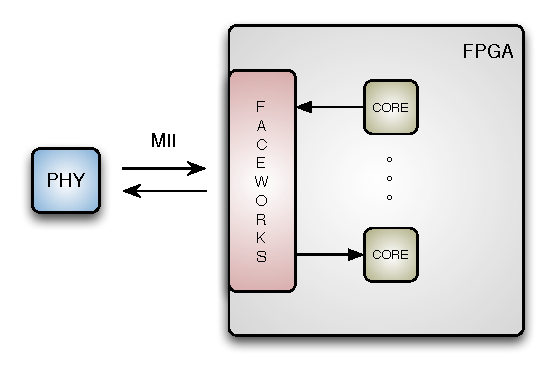
\includegraphics[scale=0.80]{Diagrams/MII.pdf}
  \caption{Interconnection of PHY and FaceWorks with MII}\label{fig:MII}
\end{figure}
\clearpage

The MII data stream is composed of the Interframe Gap (IFG), the Preamble, the Start of Frame Delimiter and the actual frame. The MAC frame is encapsulated inside the MII stream. The MAC encapsulates the payload with a 14 byte header before the data payload, followed by a 4 byte Cyclic Redundancy Check as show in Figure \ref{fig:Eth-frame}.

\begin{figure}[h]
  \centering
      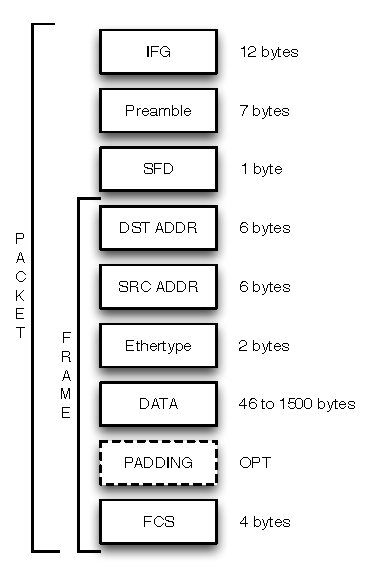
\includegraphics[scale=0.8,center]{Diagrams/MAC-FRAME.pdf}
  \caption{Ethernet packet structure with the MAC protocol}\label{fig:Eth-frame}
\end{figure}

The FaceWorks implementation of the MII interface and MAC layer consists of two logic blocks, an Ethernet receiver and an Ethernet transmitter, as shown in Figure \ref{fig:FW-diag}.

The receiver block is responsible for removing the preamble, detecting the SFD, performing packet filtering based on the destination MAC and Ethertype, and checking the CRC to validate the data.

The inverse operation is performed by the transmitter block: it adds the preamble to the payload, inserts the SFD, the Ethernet header, and calculates the trailing CRC.


\subsection{Network Layer}

The implementation of the IP protocol in FaceWorks uses two blocks, the IP RX block and the IP TX block, as depicted in Figure \ref{fig:FW-diag}. 

The IP RX block implements the IP protocol for the receive packets. It processes the IP packets that are received from the MAC layer, according to the values of their IP header version, destination IP address and protocol type. It calculates the checksum to verify the header and forwards the payload data to the next block, the UDP RX block.

For transmit packets the IP TX block calculates the header checksum and writes the IP header and checksum in the RAM TX block, which is where the packet is being formed. Finally, it requests the Ethernet TX module to send the packet.

\subsection{Transport Layer}
\begin{figure}[h]
  \centering
      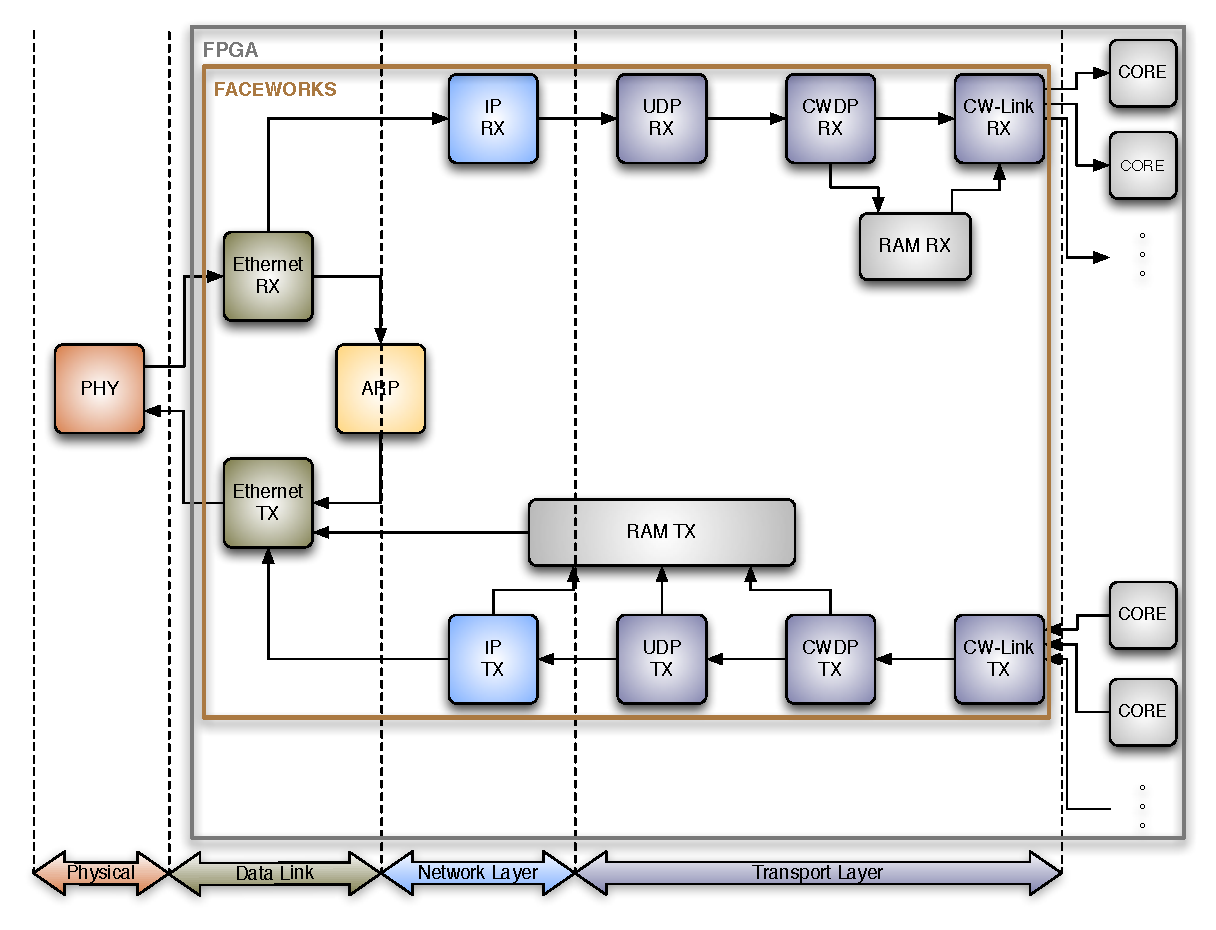
\includegraphics[width=9cm,center]{Diagrams/FW_paper.pdf}
  \caption{FaceWorks Block Diagram}\label{fig:FW-diag}
\end{figure}

The FaceWorks implementation for the transport layer is also composed of two blocks, the UDP RX and the UDP TX blocks, as shown in Figure \ref{fig:FW-diag}.

The UDP RX block filters out UDP messages that are not being sent to the UDP port being used for CWDP communication. For messages addressed to the UDP port being used for CWDP communication, the UDP RX block removes the UDP header and forwards the UDP payload (CWDP packet) to the CWDP RX module. 

The UDP TX block inserts the UDP header in the RAM TX buffer, calculates the checksum assuming the pseudo-header is attached upfront, and forwards the transmission of the UDP packet to the IP TX module.

\subsection{Coreworks Datagram Protocol}
The Coreworks Datagram Protocol (CWDP)\cite{Facedata} is a proprietary UDP based protocol created to communicate with the on-chip cores using the FaceWorks core.

\subsubsection{CWDP Packet}

Figure \ref{fig:cwdp-packet} shows how an CWDP packet is structured. The fields are briefly described below

\begin{figure}[h]
  \centering
      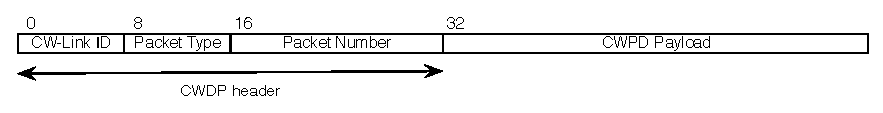
\includegraphics[width=9cm,height=1.25cm]{Diagrams/CWDP-Packet.pdf}
  \caption{CWDP packet}\label{fig:cwdp-packet}
\end{figure}

\paragraph*{CW-Link ID} This field identifies the destination core interface for which the packet data is intended.
\paragraph*{Packet Type} This field identifies the CWDP packet type; not all available packet types are used in this work.
\paragraph*{Packet Number} This field is a sequence number for data packets. It is used to implement reliable transmission. The Packet Number is incremented for every packet acknowledged by the receiver. Only packets with the expected Packet Number are acknowledged by the receiver.
\paragraph*{Payload} Contains the data to be delivered to the cores, or parameters for FaceWorks.


\subsubsection{Packet Types}

This section presents the CWDP packet types that have been used in this work. Refer to \cite{Facedata} for a complete outline of the existing CWDP packet types.

% %START CORE ACCESS
\paragraph*{SET\_CORE\_ACCESS} (packet type 0x03) This packet type is used to initialize the FaceWorks core. In Figure \ref{fig:cwdp-core-access} the structure of a CWDP SET\_CORE\_ACCESS packet is shown. When a CWDP SET\_CORE\_ACCESS packet is received by FaceWorks it locks to the host IP and UDP port of the origin for the purpose of replying. The ARP table is cleared and any packet present in the receive or transmit buffers are deleted. Incoming or outgoing packet counters are both reset to zero. The registered host will maintain control of FaceWorks core until a CWDP SET\_MAC packet is sent by the host. When FaceWorks is locked to a host, other incoming CWDP packets from other origins are dropped.

\begin{figure}[h]
  \centering
      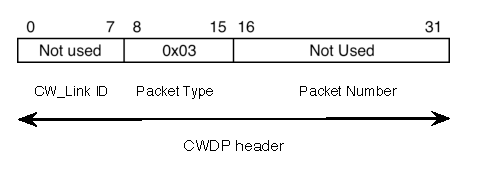
\includegraphics[height=2cm]{Diagrams/CWDP-Set-core-access.pdf}
  \caption{CWDP SET\_CORE\_ACCESS packet}
  \label{fig:cwdp-core-access}
\end{figure}

\paragraph*{SET\_MAC} (packet type 0x04) This type is now used to release control and terminate a connection with the FaceWorks core. In a complete FaceWorks implementation this could be used to change from core access mode to MAC mode. In MAC mode FaceWorks as a regular MAC core by an embedded processor and CORE\_DATA packets can not be transmitted.  In Figure \ref{fig:mac-access} the structure of the CWDP SET\_MAC packet is shown. When a CWDP SET\_MAC packet is received the control of the FaceWorks core is released, the registered IP and UDP port are deleted, the ARP table is cleared and packet buffers are cleared. Incoming or outgoing packet counters are both reset to zero. Control can be regained by sending a SET\_CORE\_ACCESS packet again.

\begin{figure}[H]
  \centering
      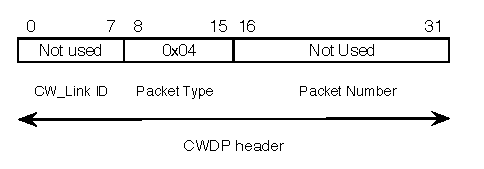
\includegraphics[height=2cm]{Diagrams/CWDP-Set-MAC.pdf}
  \caption{CWDP SET\_MAC packet}
  \label{fig:mac-access}
\end{figure}

\paragraph*{CORE\_DATA} (packet type 0x01) This packet type is used to send data between systems and cores. In Figure \ref{fig:cwdp-data} a CWDP CORE\_DATA packet is shown. The packet payload is composed of several CW-Link words, each word is 32-bit long and each CORE\_DATA packet can contain up to 360 CW-Link words.

\begin{figure}[h]
  \centering
      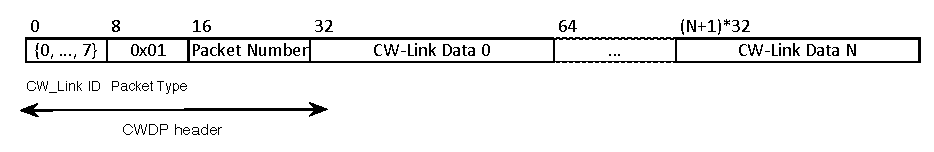
\includegraphics[width=9cm,height=2cm]{Diagrams/CWDP_Core_data_paper.pdf}
  \caption{CWDP CORE DATA packet}
  \label{fig:cwdp-data}
\end{figure}

\paragraph*{ACK} (packet type 0x02) This packet type is used to acknowledge received packets. In Figure \ref{fig:cwdp-ack}, the structure of a CWDP ACK packet is shown. Received CWDP packets, except for the ACK packet itself, trigger a reply with an ACK packet. The packet number of the transmitted ACK matches the packet number of the received packet when a CORE DATA packet is received. If the received packet is a SET\_CORE\_ACCESS packet then the packet number of the ACK packet is set to zero.

\begin{figure}[h]
  \centering
      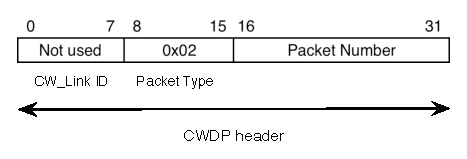
\includegraphics[height=2cm]{Diagrams/CWDP-Ack.pdf}
  \caption{CWDP ACK packet}
  \label{fig:cwdp-ack}
\end{figure}

\subsection{Implementation}

The CWDP application layer is implemented using 4 logic blocks (CWDP RX, CWDP TX, CW-Link RX and CW-Link TX), as shown in Figure \ref{fig:FW-diag}.

The CWDP RX block implements the CWDP protocol for the received packets. It decodes the type of the received packet and performs the instructed action. The payload of CORE\_DATA packets is placed in the RAM RX buffer. After the reception of a CWDP packet it requests the CWDP TX to send the acknowledge packet. If the CWDP packet is a CORE DATA packet it forwards the data to CW-Link RX block in order to be delivered to the addressed IP Core. An interaction diagram between the CWDP receive and transmit sides is shown in Figure \ref{fig:cwdp-transac}.

\begin{figure}[h]
  \centering
      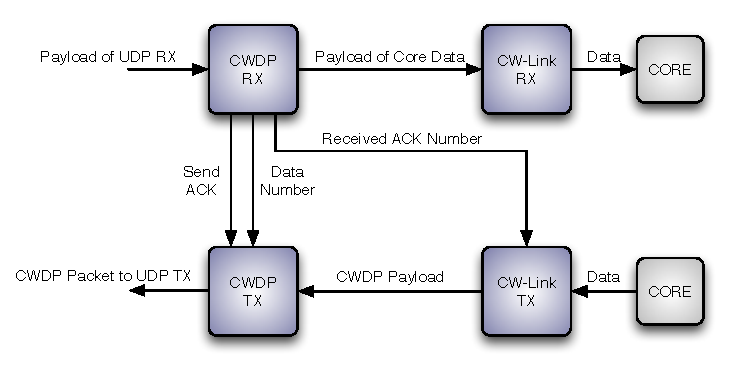
\includegraphics[scale=0.75,center]{Diagrams/CWDP-simplified-transaction.pdf}
  \caption{CWDP Layer}
  \label{fig:cwdp-transac}
\end{figure}

The CWDP TX block receives data from the CW-Link TX block and sends the data to the UDP TX module by means of the RAM TX buffer. Then it waits for the ACK packet of the sent packet, which will arrive in the CWDP RX block. When the ACK packet arrives, the CWDP RX block presents the sequence number to the CWDP TX block, so it can verify that it matches the sequence number of the packet previously sent.

\section{Design}

In this chapter the implementation of multiple UDP ports for FaceWorks is presented. The software components and the hardware modifications effected to support two distinct ports are explained. The same method can be used for more than two ports.

During the development a loopback has been used, where the CW-Link RX is directly connected to CW-Link TX is shown in Figure \ref{fig:CW-LoopBack}. With this test case, no IP cores other than FaceWorks are needed.

\begin{figure}[h]
  \centering
      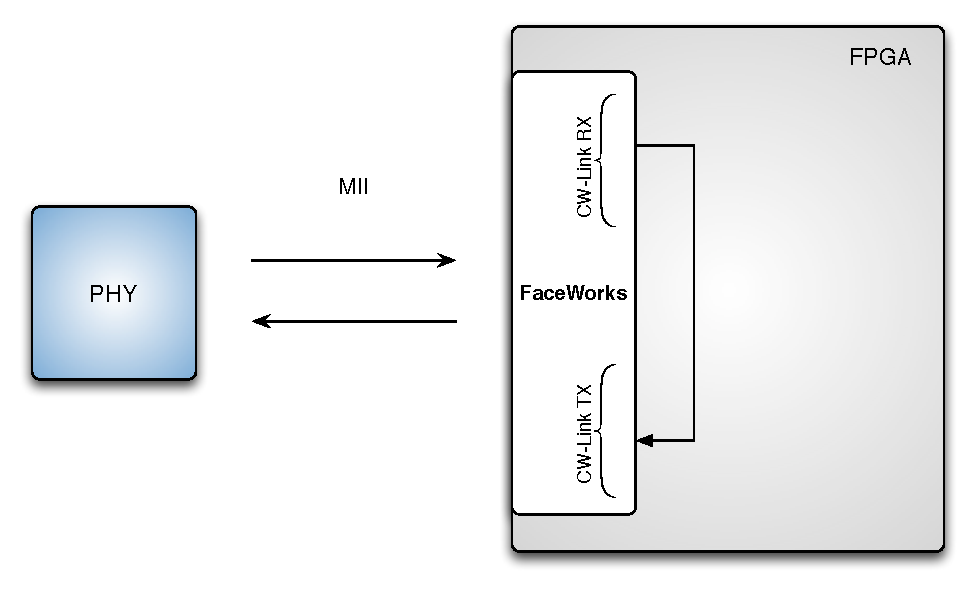
\includegraphics[width=9cm]{Diagrams/CW-LoopBack_paper.pdf}
  \caption{Cw-Link Loopback}\label{fig:CW-LoopBack}
\end{figure}

\subsection{Face-Test}

The FaceWorks test application (Face-Test) is a C language application that implements the CWDP protocol. The application has been tested on the pre-existing FaceWorks architecture and on the new FaceWorks architecture.

\paragraph*{Basic Functions}
The two basic functions used in the Face-Test application are the {\tt CWDP\_receive\_packet()} and the {\tt CWDP\_send\_packet()} functions. These functions create an abstraction layer which hides the CWDP details. They are used for sending / receiving packets to / from FaceWorks, and can be called for different sessions/connections inside a user process.

\subsection{New Hardware Implementation}

The new architecture is presented in Figure \ref{fig:FW-Final}. Compared to the original architecture, the CWDP\_Link modules are duplicated on both the reception and transmission sides. The RAM\_RX block is also duplicated in order to receive and store two consecutive packets with different destination ports. An arbiter is added to decide which of the CW-Link TX is granted access to the medium.

\begin{figure}[h]
  \centering
      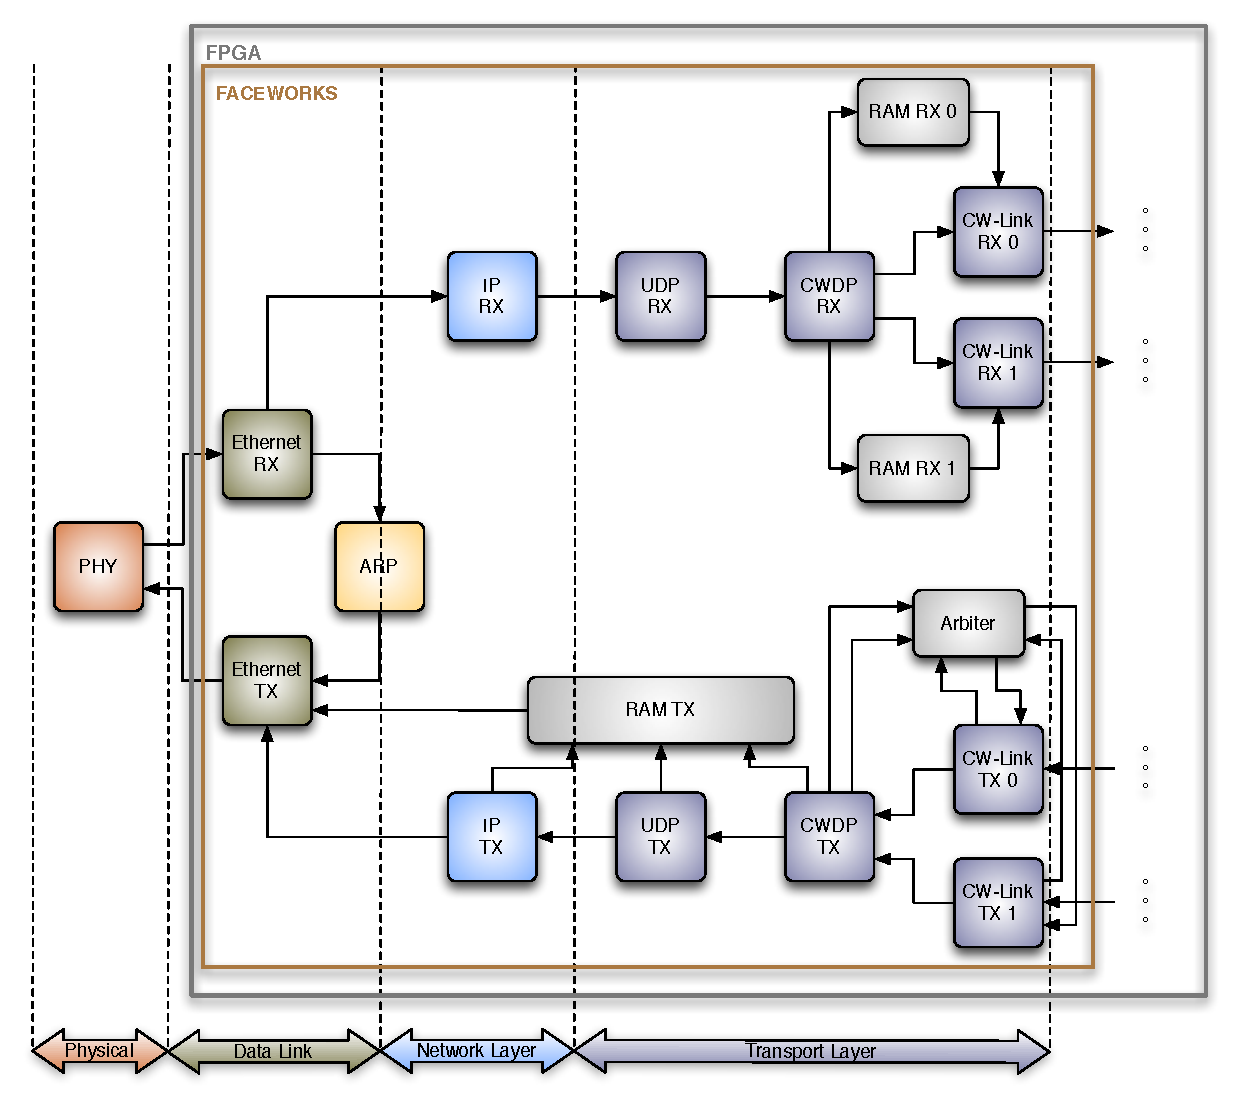
\includegraphics[width=9cm]{Diagrams/FW-Final_paper.pdf}
  \caption{Two-port FaceWorks Block Diagram}\label{fig:FW-Final}
\end{figure}

In this implementation FaceWorks supports a single sender IP address and listens to two hardwired UDP ports, whose numbers differ by 1. For example, ports 1234 and 1235. The following paragraphs describe the modifications effected on the original hardware blocks.

\paragraph*{UDP RX} The UDP RX block original implementation filtered out the UDP packets whose destination port did not match the current listening port. This behavior has been modified. The UDP destination port field is subtracted from the base listening port. If the result is 0 then the packet is aimed at the first port; if the result is 1 the packet is aimed at the second port; if the result is neither 0 nor 1 then the packet is dropped.

\paragraph*{CWDP RX} The CWDP RX block is used for both ports and it must keep track of the packet sequence numbers for the two ports. A block diagram is depicted in Figure \ref{fig:CWDPRXDETAIL}.

\begin{figure}[h]
  \centering
      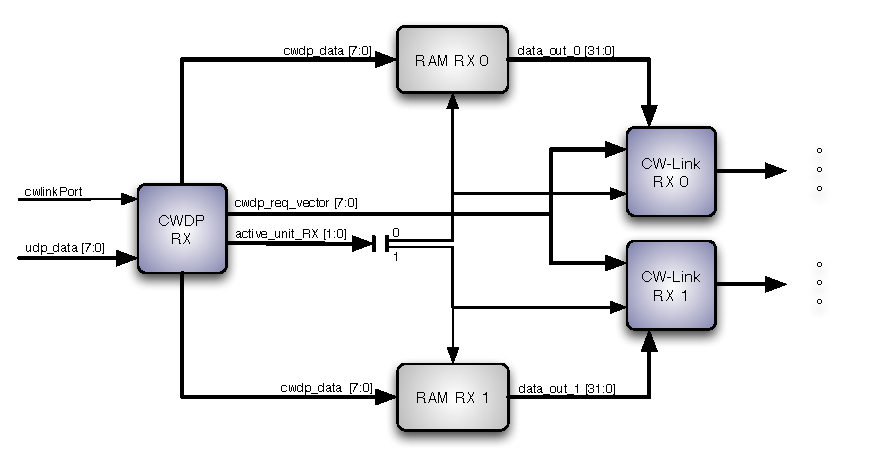
\includegraphics[width=10cm]{Diagrams/CWDP-RX-Detail.pdf}
  \caption{CWDP RX and CW-Link RX}\label{fig:CWDPRXDETAIL}
\end{figure}

The control signal {\tt CwLinkPort} produced by the UDP RX block identifies the currently active port, and is used to select the packet sequence number register to check and increment. The \texttt{CwLinkPort} signal is also decoded to produce a 2-bit signal \texttt{active\_unit\_RX} to select the active Cw-Link RX block. Upon reception of a SET\_CORE\_ACCESS packet from a given UDP port, one of two registers named {\tt( locked\_UDP\_0} and {\tt locked\_UDP\_1)} is set with the source UDP port. These are provided to the CWDP TX block so it can choose the correct destination UDP port to reply to. See Figure \ref{fig:CWDPSIMP2}.


\paragraph*{Cw-Link RX} The Cw-Link RX unit is duplicated, one for each communication port. The control FSM has been modified so that they are activated one at a time, based on the value of the control signal {\tt active\_unit\_RX}.

\begin{figure}[h]
  \centering
      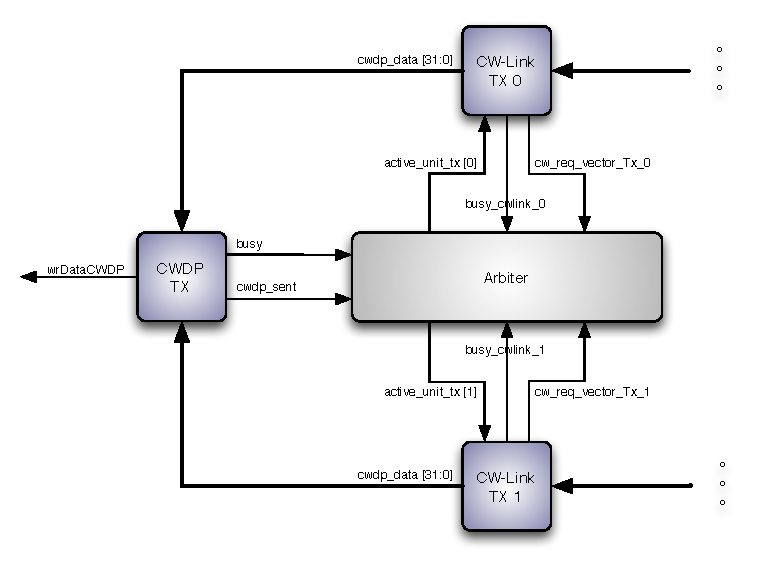
\includegraphics[width=10cm,center]{Diagrams/CWDP-TX-Detail.pdf}
  \caption{CWDP TX and CW-Link TX}\label{fig:CWDP-TX}
\end{figure}

\paragraph*{Cw-Link TX} The Cw-Link TX unit is duplicated. The control FSM has been modified to allow execution only when the Arbiter block grants access to the (RAM TX and CWDP TX) resources. To do this, two signals are sent to the arbiter \texttt{cw\_req\_vector\_TX} and \texttt{busy\_cwlink}, and one signal is received from the arbiter \texttt{active\_unit\_tx}, as shown in Figure \ref{fig:CWDP-TX}. When the resources are granted to one of the Cw-Link TX units the arbiter waits until its execution ends before granting the resources to the other Cw-Link TX unit.

\paragraph*{CWDP TX} A single CWDP TX is used. The UDP destination port may be different depending on the type of packet: ACK packet requested by the CWDP RX block or data packet requested by one of the two CW-Link TX units, as shown in Figure \ref{fig:CWDPSIMP2}. If the CWDP TX is processing a CORE\_DATA packet, the destination UDP port is selected from the \texttt{locked\_UDP\_0} or \texttt{locked\_UDP\_1} inputs, based on the currently active CW-Link TX block. For an ACK packet request, the {\tt SendACK} signal is activated, the {\tt SelACK} signal selects the UDP destination port from the \texttt{locked\_UDP\_0} or \texttt{locked\_UDP\_1} inputs, and the sequence number is provided by the {\tt SeqNumACK} signal.

\begin{figure}[h]
  \centering
      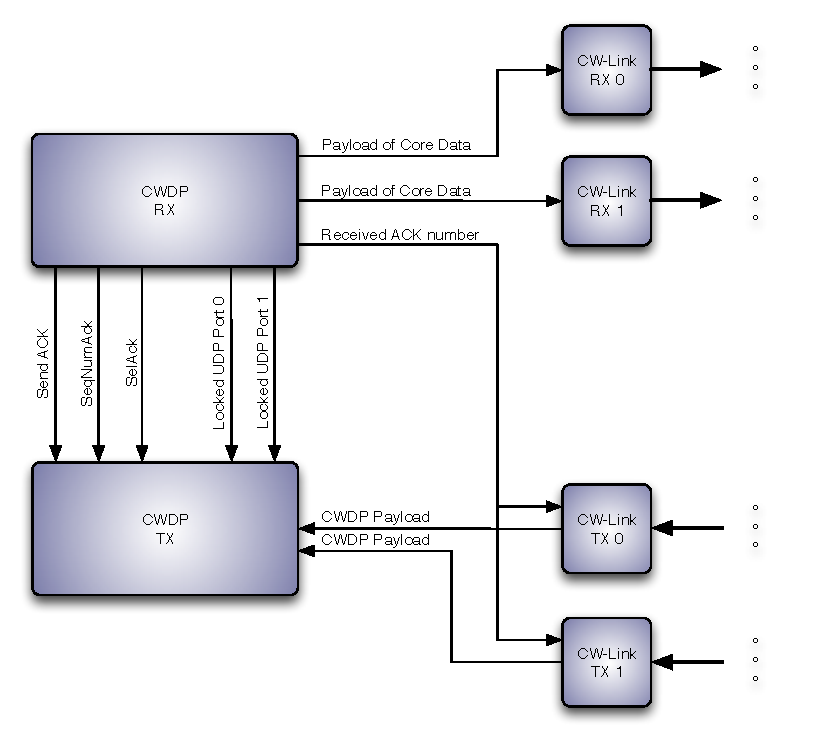
\includegraphics[width=9cm,center]{Diagrams/CWDP-simplified-transaction-2.pdf}
  \caption{CWDP Layer}\label{fig:CWDPSIMP2}
\end{figure}

\paragraph*{Arbiter} To control the access to both the CWDP TX and the RAM TX modules from the CW-Link TX modules an arbiter block has been implemented. The arbiter's algorithm is simple and tries to ensure that both UDP ports get the same priority in using FaceWorks's transmission infrastructure: when both ports want to have access to the CWDP layer, control is toggled from the port that currently has control to the port that currently does not have control.


\section{Verification}

In this chapter the methodology used to debug, verify and inspect the FaceWorks core is presented. 

Initially, verification of the design was being performed directly on the FPGA using as main tools for debug a packet sniffer (Wireshark), an ILA (Xilinx's ChipScope Pro) and the Face-Test application to send stimuli to the FPGA board and analyze the responses. However, as the design got near completion, some intermittent bugs showed up, which were very difficult to identify using this ad-hoc verification method.

The main difficulty was to know when and what signal was the causing a problem, so that correct trigger conditions could be set. Using the ILA proved ineffective due to too many inconclusive trigger conditions, and a limited buffer size to store data samples for analysis, which is the result of having limited number of BRAM in the device. 

An alternative consisted in creating a testbench and running the system into a simulator such Xilinx's iSim. However, it was difficult to recreate realistic test conditions, unless a significant amount of C and Verilog code were developed. Another way is to modify the system in order to be able to run a simpler to write testbench, but this approach is risky as important features may end up untested.

Besides, methods for the testbench to read and write data are limited to file IO since no Verilog Procedural Interface (VPI) support is offered for iSim. Writing and reading files to exercise the MII interface in a testbench is hard and complicated to implement, considering the sheer amount of data needed to adequately test a network interface.  So other alternatives were searched so that the design could be properly debugged and verified. Of the considered alternatives, Verilator, a free open source application, has been chosen to perform this task.

\subsection{Verilator}

Verilator is an application that translates a synthesizable Verilog description into an optimized cycle-accurate behavioral model in C++/SystemC, which is called a verilated file. Verilator is a two state simulator (0,1), but it has features to deal with unknown states. The testbench is a C/C++ application that wraps the verilated model and is compiled with it using a common C++ compiler. Verilated models show high simulation speed, which is on par or higher than commercial simulators such as NC-Verilog, VCS and others. \cite{veribench}.

\subsection{A Testbench for FaceWorks}

%Verificar a consistência de todos os títulos: se letras maisúcuilas são usadas então que seja em todos.

Using Verilator, a FaceWorks simulator has been created which can be stimulated with the same socket-based test application used for exercising FaceWorks in an FPGA. In this way test patterns that fail in the FPGA device can be replicated and analyzed in simulation with full visibility over all design signals. A FaceWorks SystemC model is created by running Verilator on the FaceWorks Verilog code, and this object is then instantiated in the testbench application.

\subsection{Testbench Implementation}


\begin{figure}[h]
  \centering
      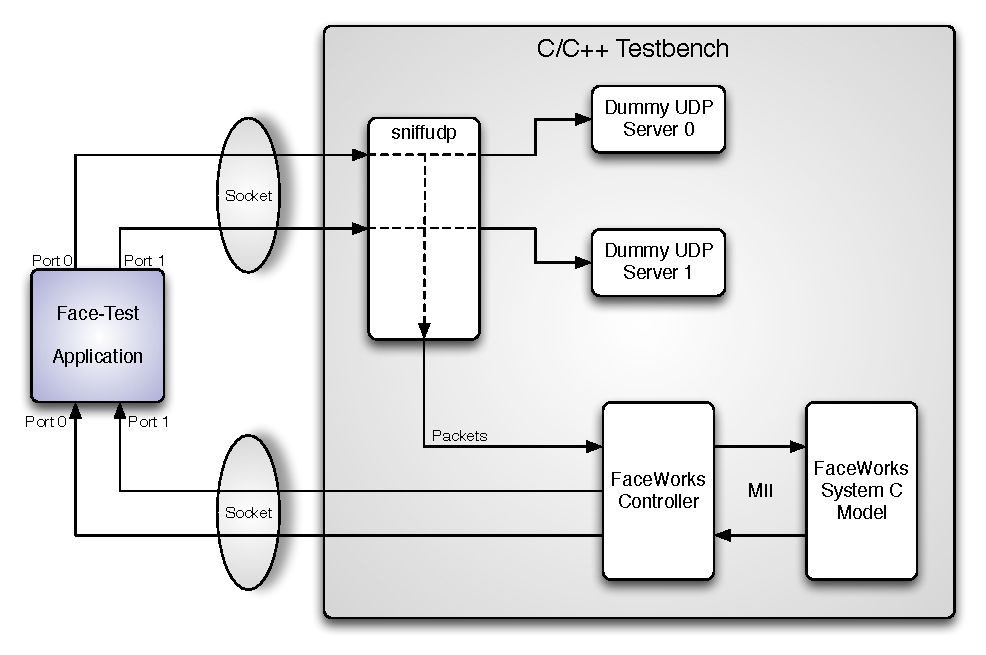
\includegraphics[scale=0.5,center]{Diagrams/TestBench-Diag.pdf}
  \caption{Verification Environment }\label{fig:tbschem}
\end{figure}

%mudar o nome das dummy udp threads de modo a ter figuras e texto consistentes.


Figure \ref{fig:tbschem} shows the verification environment for FaceWorks, encompassing the Face-test application and the C++ testbench. The testbench has five components: 3 threads (\texttt{Dummy UDP Server 0}, \texttt{Dummy UDP Server 1} and {\tt sniffudp}), the FaceWorks Controller, and the FaceWorks model.

The two threads \texttt{Dummy UDP Server 0} and \texttt{Dummy UDP Server 1} perform the simple operation of reading the UDP ports persistently, so the input data coming from the application do not fill the OS socket buffer.

The {\tt sniffudp} thread launches the data capture code, which is based on the sniffex.c code example of {\tt libcap}, a portable C/C++ library for network traffic capture \cite{sniffer}. 

This data capture code must be used instead of a simple UDP socket, because this way the full Ethernet frame is captured, which makes it easier to reconstruct the MII packet in order to feed the data to the MII interface of the FaceWorks model.

The FaceWorks Controller is responsible for receiving data from the \texttt{sniffudp} thread, formatting the data according to the MII format and deliver them to the FaceWorks MII interface. The FaceWorks Controller is also responsible for unpacking the data it receives from the FaceWorks model in order do send them to the test application via UDP sockets.

The FaceWorks model is a SystemC Model created by running Verilator on the FaceWorks Verilog code.

Threads are used so that the FaceWorks Controller can run at the same time as data is intercepted by the {\tt sniffudp} function. These two components are explained in detail in the next two subsections.

\subsection{sniffudp}

A simpler solution to capture data from the Face-Test application is to implement a C/C++ UDP socket server in the testbench to read the incoming data from the Face-Test application and provide it to the FaceWorks SystemC model. However, since the FaceWorks connection to the outside is the MII interface, one would need to recreate the MII packet from the received UDP payload. Recreating the MII packet implies recreating the UDP packet followed by the IP packet, followed the Ethernet frame. This would be unnecessarily complicated.

A solution for this problem is to capture the packets at the data link layer, which can be accomplish by the use of \texttt{libpcap}, avoiding the process of recreating the Ethernet, IP and UDP packets.

The \texttt{sniffudp} function is set to capture data on the Linux loopback ({\tt lo}) device, which are addressed with the two FaceWorks UDP ports. The {\tt lo} device is a virtual network interface used to receive packets sent from the host to itself. After the setup the \texttt{sniffudp} thread blocks waiting for filtered packets. When such packets arrive they are passed to a callback function \texttt{got\_packet()}.

The \texttt{got\_packet()} function receives almost complete Ethernet frames (Figure \ref{fig:Eth-frame}) which miss the FCS field and have a blank destination and source address, since the data is traveling through the loopback interface. The fields preamble, SFD, destination address, source address and Ethertype are inserted. The data field (containing the IP packet) is copied from the sniffed packet. The CRC is calculated as described in section \ref{subsec:CRC} and appended as the FCS field.

Then, the \texttt{got\_packet()} function reaches a critical region where it pushes the packet into a queue shared with the main thread, after which it terminates execution. When another packet is filtered the callback function is called again and the process repeats all over again.


\subsection{FaceWorks Controller}

The FaceWorks Controller instantiates the FaceWorks model, and communicates with it. Since the FaceWorks Controller does not implement the ARP protocol, to properly support the communication between the Face-Test application and the FaceWorks model, the FaceWorks controller starts by sending a fixed ARP reply packet as shown in Figure \ref{fig:Arp-packet}. This packet is sent even without receiving any ARP request from the FaceWorks model. The purpose is to fill the ARP cache with an IP address / MAC address pair, so the FaceWorks Ethernet TX module can obtain the MAC address  by consulting the ARP module. If the cache is already stuffed, no ARP query packets will be generated by the FaceWorks model.

\begin{figure}[h]
  \centering
      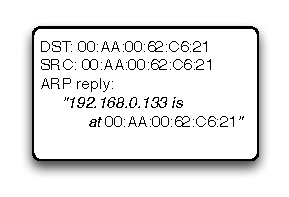
\includegraphics[scale=.8,center]{Diagrams/ARP-stuffing.pdf}
  \caption{Injected ARP Reply Packet }\label{fig:Arp-packet}
\end{figure}

After the ARP stuffing is completed, the FaceWorks controller is in a loop, trying to transfer data from the packet queue, shared with the \texttt{sniffudp} thread, to the MII RX interface of the FaceWorks model, and/or to transfer data from the MII TX interface to the socket that leads to the Face-Test application.

To transfer data from the queue to the MII RX interface the FaceWorks controller needs to get hold of the mutex that protects the shared packet queue. When access to the mutex is granted and at least one packet exists in the queue, the packet is popped from the queue and fed into the MII RX interface of the FaceWorks model, nibble by nibble.

To transfer data to the socket leading to Face-Test, the FaceWorks controller  stores the received nibbles in a buffer, which is then passed to another function, the \texttt{process\_recv\_packet} function discussed in the next section, which verifies and forwards the data to the Face-Test application.


\subsection{process\_recv\_packet}
\label{subsec:process_recv}

The \texttt{process\_recv\_packet} function receives as argument a packet buffer from the FaceWorks controller, processes the packet and sends it over the network socket to the Face-Test application.

The \texttt{process\_recv\_packet} function checks if the Preamble, SFD and Ethernet headers are correctly constructed, by comparing their values to the expected values. The FCS field is calculated for the received packet and compared with the FCS value in the packet itself. The FCS field contains a CRC checksum computed as described in section \ref{subsec:CRC}. If any field does not match the expected value, the function returns with an error which indicates the malformed field.

If a well formed packet is received, the IP headers and UDP headers are read to extract the destination IP address, UDP port and UDP payload offset, and the UDP packet is sent to the Face-Test Application.

By verifying the data from the MII interface, the operation of the FaceWorks model is always under scrutiny, which is a valuable debug feature. Next, the Ethernet, IP and UDP headers are removed,  and the data is placed into the UDP socket to be sent to the Face-Test application, which is listening to the UDP ports in use.

\subsection{Cyclic Redundancy Check}
\label{subsec:CRC}
The CRC is computed by both the \texttt{process\_recv\_packet} and the \texttt{got\_packet} function. The source code used to calculate the CRC has been generated by a Python script denominated \texttt{pycrc}\cite{pycrc}. The \texttt{pycrc} script outputs a C header file (.h) and C source code file (.c) which can compute the CRC.

\section{Results}

In this chapter two kind of results are presented: 1) FPGA implementation results on consumed resources and operation frequency; 2) bandwidth results.

\subsection{FPGA Implementation Results}

The system has been developed and tested on a Xilinx SP605 board, featuring a Spartan 6 XC6SLX45T device and a Marvell Alaska PHY (88E1111) chip. The Spartan 6 is a low end device, designed for larger production volumes and low price but with limited performance.

\begin{table}[h]
\centering
\caption{Implementation Results for the Single-Port FaceWorks}
\label{table:Implementation Results of the single port FaceWorks}
\begin{tabular}{c c c c}
\hlinew{0.08cm}
\cellformatrG{}&\cellformatlrG{}&\cellformatlrG{}&\cellformatlG{}\\
\cellformatrG{\multirow{-2}{7 cm}{}} &
\cellformatlrG{\multirow{-2}{2cm}{\centering Used}}&
\cellformatlrG{\multirow{-2}{1.8cm}{\centering Total}}&
\cellformatlG{\multirow{-2}{2cm}{\centering Percentage Used}}
\\
\hlinew{0.08cm}
\greyrow \multicolumn{4}{c}{Slice Logic Utilization}
\\
\hlinew{0.04cm}
\cellformatrW{\-\hspace{0.5cm}Number of Slice Registers\hfill } & \cellformatlrW{1527} & \cellformatlrW{54576} & \cellformatlW{2\%}\\
\cellformatrW{Number of Slice LUTs:\hfill} & \cellformatlrW{2178} & \cellformatlrW{27288} & \cellformatlW{7\%}\\
\cellformatrW{\hfill Number used as Logic} & \cellformatlrW{2036} & \cellformatlrW{27288} & \cellformatlW{7 \%}\\
\cellformatrW{\hfill \-\hspace{1.5cm}Number used as Memory} & \cellformatlrW{16} & \cellformatlrW{6048} & \cellformatlW{1 \%}\\
\hlinew{0.08cm}
\greyrow \multicolumn{4}{c}{Slice Logic Distribution}
\\
\hlinew{0.04cm}
\cellformatrW{Number of LUT Flip Flop pairs used:\hfill } & \cellformatlrW{2375} & \cellformatlrW{-} & \cellformatlW{-}\\
\cellformatrW{\-\hspace{2cm}Number with an unused Flip Flop} & \cellformatlrW{999} & \cellformatlrW{2375} & \cellformatlW{42\%}\\
\cellformatrW{\-\hspace{1.3cm}Number with an unused LUT\hfill} & \cellformatlrW{197} & \cellformatlrW{2375} & \cellformatlW{8 \%}\\
\cellformatrW{\-\hspace{2.2cm}Number of fully used LUT-FF pairs\hfill} & \cellformatlrW{1179} & \cellformatlrW{2375} & \cellformatlW{49 \%}\\
\hlinew{0.08cm}
\greyrow \multicolumn{4}{c}{Specific Feature Utilization}
\\
\hlinew{0.04cm}
\cellformatrW{Number of Block RAM (16Kb)} & \cellformatlrW{2} & \cellformatlrW{116} & \cellformatlW{2\%}\\
\hlinew{0.08cm}


\end{tabular}
\end{table}



The synthesis results presented are obtained with the Xilinx ISE 14.4 suite of tools. In Table \ref{table:Implementation Results of the single port FaceWorks}, synthesis results for the original single port implementation are presented. Table \ref{table:Implementation Results of the two port FaceWorks} presents synthesis results for the two-port implementation designed in this work.


\begin{table}[h]
\centering
\caption{Implementation Results for the Two-Port FaceWorks}
\label{table:Implementation Results of the two port FaceWorks}
\begin{tabular}{c c c c}
\hlinew{0.08cm}
\cellformatrG{}&\cellformatlrG{}&\cellformatlrG{}&\cellformatlG{}\\
\cellformatrG{\multirow{-2}{7 cm}{}} &
\cellformatlrG{\multirow{-2}{2cm}{\centering Used}}&
\cellformatlrG{\multirow{-2}{1.8cm}{\centering Total}}&
\cellformatlG{\multirow{-2}{2cm}{\centering Percentage Used}}
\\
\hlinew{0.08cm}
\greyrow \multicolumn{4}{c}{Slice Logic Utilization}
\\
\hlinew{0.04cm}
\cellformatrW{\-\hspace{0.5cm}Number of Slice Registers\hfill } & \cellformatlrW{1917} & \cellformatlrW{54576} & \cellformatlW{3\%}\\
\cellformatrW{Number of Slice LUTs:\hfill} & \cellformatlrW{2965} & \cellformatlrW{27288} & \cellformatlW{10\%}\\
\cellformatrW{\hfill Number used as Logic} & \cellformatlrW{2933} & \cellformatlrW{27288} & \cellformatlW{10 \%}\\
\cellformatrW{\hfill \-\hspace{1.5cm}Number used as Memory} & \cellformatlrW{32} & \cellformatlrW{6048} & \cellformatlW{1 \%}\\
\hlinew{0.08cm}
\greyrow \multicolumn{4}{c}{Slice Logic Distribution}
\\
\hlinew{0.04cm}
\cellformatrW{Number of LUT Flip Flop pairs used:\hfill } & \cellformatlrW{3963} & \cellformatlrW{-} & \cellformatlW{-}\\
\cellformatrW{\-\hspace{2cm}Number with an unused Flip Flop} & \cellformatlrW{2046} & \cellformatlrW{3963} & \cellformatlW{51\%}\\
\cellformatrW{\-\hspace{1.3cm}Number with an unused LUT\hfill} & \cellformatlrW{998} & \cellformatlrW{3963} & \cellformatlW{25 \%}\\
\cellformatrW{\-\hspace{2.2cm}Number of fully used LUT-FF pairs\hfill} & \cellformatlrW{919} & \cellformatlrW{3963} & \cellformatlW{23 \%}\\
\hlinew{0.08cm}
\greyrow \multicolumn{4}{c}{Specific Feature Utilization}
\\
\hlinew{0.04cm}
\cellformatrW{Number of Block RAM (16Kb)} & \cellformatlrW{3} & \cellformatlrW{116} & \cellformatlW{2\%}\\
\hlinew{0.08cm}


\end{tabular}
\end{table}



The synthesis results show that both FaceWorks designs are very economic in terms of size. However, it must be noted that the single-port design only supports 8 CW-Link connections, while the two-port design supports 16 CW-Link connections. The IP cores use very little memory and zero DSP blocks. The overall size can be considered adequate for a test and debug core. For a small FPGA like the Spartan 6 , it only occupies 10 \% of the logic resources in the two-port configuration. 

The results show that with about 7000 gates  a new UDP port and 8 new CW-Link connections can be added to the design. Thus, the design scales almost linearly, being the non-linear part the small amount of logic needed to augment the size of the arbiter.

\begin{table}[h]
\centering
\caption{Period Timing Constraints}
\label{table:Timing Constratints of the Dual Port FaceWorks}
\begin{tabular}{c c c}
\hlinew{0.08cm}
\cellformatrG{}&\cellformatlrG{}&\cellformatlG{}\\
\cellformatrG{\multirow{-2}{*}{\centering }} &
\cellformatlrG{\multirow{-2}{2cm}{\centering Used}}&
\cellformatlG{\multirow{-2}{1.8cm}{\centering Minimum}}
\\
\hlinew{0.04cm}
\cellformatrW{ Sys\_clk } & \cellformatlrW{20 ns} & \cellformatlW{8.341 ns}\\
\cellformatrW{ TX\_CLK } & \cellformatlrW{40 ns} & \cellformatlW{ NA }\\
\cellformatrW{ RX\_CLK } & \cellformatlrW{40 ns} & \cellformatlW{ NA }\\
\end{tabular}
\end{table}

The system clock period used and the minimum period constraint that has been possible to meet are shown in Table  \ref{table:Timing Constratints of the Dual Port FaceWorks}. The minimum period (8.341 ns), which corresponds to about 120MHz is a competitive frequency for a Spartan 6 device. Compared to the single port implementation, where the minimum clock period is 6.912 ns, the minimum clock period increases 20\% for the two-port implementation. This is mostly due the Arbiter block design, which scales poorly in terms of frequency. A better design would not be very difficult to implement but falls out of the scope of this thesis. For a number of ports higher than two, it is highly recommended that the Arbiter design is reviewed.

\subsection{Ethernet Switch Characterization}

The results presented in this work have been obtained on a notebook with an Intel U4100 @ 1.30GHz processor, 3 GB of RAM and an Atheros AR8131 ethernet adapter, running the Linux kernel 3.2.0-x86-64. To interconnect Ethernet devices a TP-Link TL-WR841N switch has been used. Two network tests have been performed to the determine the switch capabilities, and detect if in either case they could limit the FaceWorks performance.

The first test was designed to determine the maximum throughput achievable with the switch. This test consisted in exchanging data in both directions, simultaneously, between two notebooks interconnected via the switch.

The throughput values presented in Table \ref{table:TL-WR841N 10/100 Mb Maximum Raw Throughput} represent raw values obtained using a random stream, without sending acknowledge packets, and without any data dependencies on the data sent by the other peer. Throughput values are measured for upstream, downstream and aggregate (sum of upstream and downstream). In the remainder of this work, the aggregate throughput obtained is used as a reference.

\begin{table}[h]
\centering
\caption{TL-WR841N 10/100 Mbps Maximum Raw Throughput}
\label{table:TL-WR841N 10/100 Mb Maximum Raw Throughput}
\begin{tabular}{c c c c}
\hlinew{0.08cm}
\cellformatrG{}&\cellformatlrG{}&\cellformatlrG{}&\cellformatlG{}\\
\cellformatrG{\multirow{-2}{*}{\centering }} &
\cellformatlrG{\multirow{-2}{2cm}{\centering Downstream}}&
\cellformatlrG{\multirow{-2}{1.8cm}{\centering Upstream}}&
\cellformatlG{\multirow{-2}{1.8cm}{\centering Aggregate}}
\\
\hlinew{0.04cm}
\cellformatrW{Throughput} & \cellformatlrW{94.54 Mbps} & \cellformatlrW{95.88 Mbps }& \cellformatlW{190.42 Mbps }\\
\hlinew{0.08cm}
\multicolumn{4}{c}{\vspace*{-0.3cm}}\\

\end{tabular}
\end{table}

These results show that in practice a throughput close to the nominal network speed has been achieved. One can say the setup introduces a 5\% degradation compared to ideal conditions.

The second test consisted in measuring the effective throughput for various packet sizes. Using the {\tt ping} application 10 packets were sent with three distinct data sizes, 54 bytes, 720 bytes and 1440 bytes. The RTT values as reported by the {\tt ping} application and effective throughput for 3 packet sizes are presented in Table \ref{table:TL-WR841N 10/100 Mbps Latency and Throughput}, where the aggregate throughput is calculated using the following expression:

\begin{equation}
Throughput = {(2 * Packet Size * 8) \over {RTT . 10^{6}}}
\end{equation}

These results show that the factor limiting the system performance is the latency. The data is packetized and a latency penalty is incurred for each packet sent. Naturally, the penalty decreases with the packet size,\begin{table}[h]
\centering
\caption{Effective Throughput}
\label{table:TL-WR841N 10/100 Mbps Latency and Throughput}
\begin{tabular}{c c c c}
\hlinew{0.08cm}
\cellformatrG{}&\cellformatlrG{}&\cellformatlrG{}&\cellformatlG{}\\
\cellformatrG{\multirow{-2}{*}{\centering Packet Size }} &
\cellformatlrG{\multirow{-2}{2cm}{\centering Latency}}&
\cellformatlrG{\multirow{-2}{1.8cm}{\centering Throughput}}&
\cellformatlG{\multirow{-2}{1.8cm}{\centering Utilization}}
\\
\hlinew{0.04cm}
\cellformatrW{54 bytes } & \cellformatlrW{0.593 ms} & \cellformatlrW{ 1.51 Mbps } & \cellformatlW{ $<$1\% }\\
\cellformatrW{720 bytes } & \cellformatlrW{0.84 ms} & \cellformatlrW{ 13.71 Mbps } & \cellformatlW{ 7.2\% }\\
\cellformatrW{1440 bytes} & \cellformatlrW{1.107 ms} & \cellformatlrW{ 20.81 Mbps }& \cellformatlW{ 10.9\% }\\
\hlinew{0.08cm}
\multicolumn{3}{c}{\vspace*{-0.3cm}}\\

\end{tabular}
\end{table}
 but even for the maximum packet size allowed by the CWDP protocol (1440 bytes), the obtained practical upper bound for the aggregate throughput (21 Mbps) is only about 11\% of the maximum possible throughput.



\subsection{Throughput Upper Bound Model}

Since no alternative paths exist in the network one can say that the OWD is approximately $OWD={RTT\over 2}$. Table \ref{table:One Way Delay} shows OWD values for the considered packet sizes.

\begin{table}[h]
\centering
\caption{One Way Delay}
\label{table:One Way Delay}
\begin{tabular}{c c}
\hlinew{0.08cm}
\cellformatrG{}&\cellformatlG{}\\
\cellformatrG{\multirow{-2}{*}{\centering Packet Size}}&
\cellformatlG{\multirow{-2}{2cm}{\centering Delay}}
\\
\hlinew{0.04cm}
\cellformatrW{54 bytes} & \cellformatlW{0.297 ms}\\
\hlinew{0.04cm}
\cellformatrW{720 bytes} & \cellformatlW{0.42 ms}\\
\hlinew{0.04cm}
\cellformatrW{1440 bytes} & \cellformatlW{0.554 ms}\\
\hlinew{0.08cm}
\end{tabular}
\end{table}

Using the OWD values, one can calculate lower bound delays for data transactions in the cases of single and double ports. The expression  {\it practical lower bound} is used because the delays measured below were always above these calculations.  This model takes into account the handshaking implemented with the small acknowledge packets. Figure \ref{fig:singleport} shows the calculation of the practical lower bound for a single-port FaceWorks system. Sending and receiving back a CORE\_DATA packet takes 1.7 ms.

\begin{figure}[h]
  \centering
      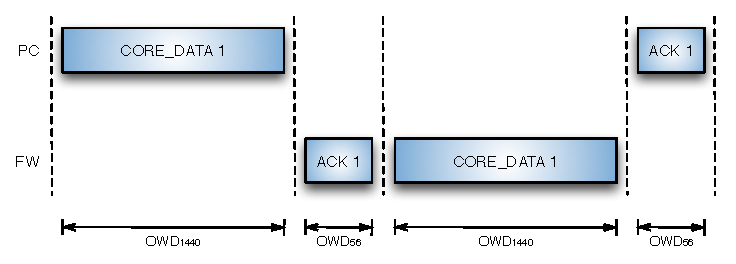
\includegraphics[width=9cm,center]{Diagrams/Single-time.pdf}
  \caption{Single Port Time Diagram}\label{fig:singleport}
\end{figure}

Figure \ref{fig:dualport} shows the calculation of the practical upper bound for a two-port FaceWorks system. Two simultaneously working ports can send and receive back two CORE\_DATA packets in approximately 2.424 ms. The blue color represents the first port, and the red color the second port.

\begin{figure}[h]
  \centering
      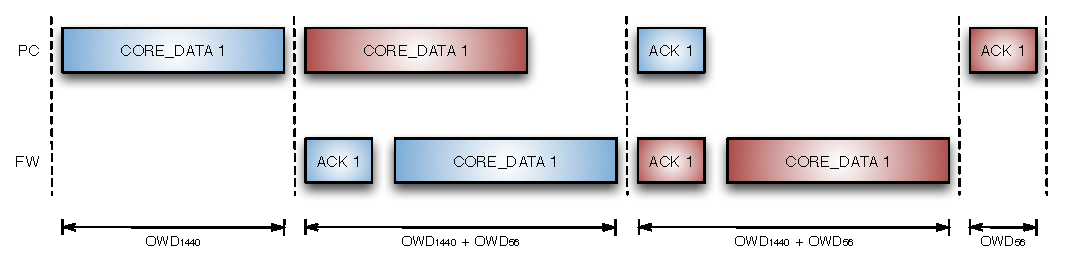
\includegraphics[width=9cm,center]{Diagrams/Dual-time.pdf}
  \caption{Dual Port Time Diagram}\label{fig:dualport}
\end{figure}

\begin{table}[h]
\centering
\caption{Throughput Model}
\label{table:Latency Model Throughput}
\begin{tabular}{c c c}
\hlinew{0.08cm}
\cellformatrG{}&\cellformatlrG{}&\cellformatlG{}\\
\cellformatrG{\multirow{-2}{*}{\centering }}&
\cellformatlrG{\multirow{-2}{2cm}{\centering Throughput}}&
\cellformatlG{\multirow{-2}{2cm}{\centering Utilization}}
\\
\hlinew{0.04cm}
\cellformatrW{Single Port} & \cellformatlrW{13.55 Mbps} & \cellformatlW{7.11\%}\\
\hlinew{0.04cm}
\cellformatrW{Dual Port} & \cellformatlrW{19.00 Mbps} & \cellformatlW{10\%}\\
\hlinew{0.08cm}
\end{tabular}
\end{table}

Converting lower bound delays to upper bound throughput yields the upper bound throughput results shown in Table \ref{table:Latency Model Throughput}. These results are considerably lower than the switch limits shown in Table \ref{table:TL-WR841N 10/100 Mb Maximum Raw Throughput}. This is made clear by column Utilization in the table, which shows the obtained throughput divided by the maximum possible throughput.  The explanation for the low utilization rate lies, firstly, in the system latency, and secondly, in the inter packet dependency between the CORE\_DATA packets and the ACK packets.

These results show that the handshaking has a dramatic effect on a single-port FaceWorks, as the next packet can only be sent after the acknowledge for the previous packet is received. The model predicts only about 14 Mbps of effective throughput using a single port.

The situation improves considerably when the second port is added, since a packet for the second port
can be sent without waiting for the acknowledge of the packet sent to the first port. The model
predicts 19 Mbps of effective throughput, which is close to the 21 Mbps limit obtained without handshaking.

\subsection{FaceWorks Sustained Throughput}


For the sustained\footnote{In networking the term {\it sustained} is used for results obtained by averaging over long periods of time.} throughput measurement, the previously benchmarked TP-Link TL-WR841N 10/100 Mbps switch has been used to interconnect the notebook and the FPGA board containing the FaceWorks core. In the FPGA, the CW-link RX-TX loopback shown in Figure \ref{fig:CW-LoopBack} was in place, so that the tests could be done using FaceWorks alone. Table \ref{table:Faceworks Throughput Results} summarizes the results obtained.

\begin{table}[h]
\centering
\caption{FaceWorks Throughput Results}
\label{table:FaceWorks Throughput Results}
\begin{tabular}{c c c c}
\hlinew{0.08cm}
\cellformatrG{}&\cellformatlrG{}&\cellformatlrG{}&\cellformatlG{}\\
\cellformatrG{\multirow{-2}{*}{\centering }} &
\cellformatlrG{\multirow{-2}{2cm}{\centering Single Port}}&
\cellformatlrG{\multirow{-2}{1.8cm}{\centering Dual Port}}&
\cellformatlG{\multirow{-2}{1.8cm}{\centering Gain}}
\\
\hlinew{0.04cm}

\cellformatrW{Original FaceWorks} & \cellformatlrW{9.86 Mbps} & \cellformatlrW{-} & \cellformatlW{-}\\
\cellformatrW{Current FaceWorks} & \cellformatlrW{11.02 Mbps} & \cellformatlrW{14.71 Mbps} & \cellformatlW{33\%}\\
\cellformatrW{Verilator Model } & \cellformatlrW{42.27 Mbps} & \cellformatlrW{79.59 Mbps}& \cellformatlW{88\%}\\
\hlinew{0.08cm}
\multicolumn{4}{c}{\vspace*{-0.3cm}}\\

\end{tabular}
\end{table}


Besides being possible to use two distinct process to control the FaceWorks, a considerable bandwidth gain is achieved when using the two ports simultaneously. 
The Verilator model bandwidth is the bandwidth calculated from the verilator model interaction with the Face-Test application with 0 latency, this only takes into account the processing overhead of the FaceWorks, and the MAC protocol. This proves that latency has a serious effect in struggling the maximum attainable throughput.

\begin{table}[h]
\centering
\caption{Measured vs. Modeled Throughput}
\label{table:Faceworks Throughput Comparision}
\begin{tabular}{c c c c}
\hlinew{0.08cm}
\cellformatrG{}&\cellformatlrG{}&\cellformatlrG{}&\cellformatlG{}\\
\cellformatrG{\multirow{-2}{*}{\centering }} &
\cellformatlrG{\multirow{-2}{2cm}{\centering Measured}}&
\cellformatlrG{\multirow{-2}{1.8cm}{\centering Model}}&
\cellformatlG{\multirow{-2}{1.8cm}{\centering Deviation}}
\\
\hlinew{0.04cm}

\cellformatrW{Single Port} & \cellformatlrW{11.02 Mbps} & \cellformatlrW{13.55 Mbps} & \cellformatlW{19\%}\\
\cellformatrW{Dual Port} & \cellformatlrW{14.71 Mbps} & \cellformatlrW{19.00 Mbps} & \cellformatlW{23\%}\\
\hlinew{0.08cm}
\multicolumn{4}{c}{\vspace*{-0.3cm}}\\

\end{tabular}
\end{table}

The values obtained by the current FaceWorks implementation are compared with the values presented in the Latency Model, which are presented in Table \ref{table:Faceworks Throughput Comparision}.

The deviation values are due to the time the computer takes to perform the operations necessary to process the packets including all the operating system processing time. Which can be considered an extra overhead on the latency.

% %%%%%%%%%%%%%%%%%%%%%%%%%%%%%%%%%%%%%%%%%%%%%%%%%%%%%%%%%%%%%%%%%%%%%%
% Conclusion
% %%%%%%%%%%%%%%%%%%%%%%%%%%%%%%%%%%%%%%%%%%%%%%%%%%%%%%%%%%%%%%%%%%%%%%
\section{Conclusion}

The design of a new multiple port FaceWorks architecture was the main objective of this work, which has been fully accomplished, including its verification and experimental characterization. 

In the hardware implementation, the UDP and CWDP modules have been modified to work with two ports. The number of CW-Link interfaces has been duplicated, in order to keep the number of debug interfaces per UDP port. Originally FaceWorks was written in the VHDL language. In this work the code was rewritten in Verilog to allow the new developments to be done also in Verilog. Besides being a lot more common in the industry, the use of Verilog was mandatory to be able to use the Verilator simulator, a key tool which made possible the completion of this project in time.

For verification a cutting-edge approach has been used. Instead of using a standard Verilog testbench and simulator, the Verilator simulator has been used to create a SystemC model of the FaceWorks design, which has been embedded in a C/C++ testbench. This solves the classical problem of integrating software and hardware in a simulation environment. Other advantages of using Verilator are the detailed linting it effects on the Verilog code, the exhaustive dumping of wave traces for debugging purposes, and the detailed coverage metrics it extracts from the design simulation. 

The design has been synthesized and tested in a Xilinx Spartan 6 FPGA. The implementation proved small and fast enough for a debug core, as such cores should not take too much space in the overall system design.

First the characterization of the used Ethernet switch was done to have practical upper bounds for bandwidth, instead of the nominal 100 Mbps. From a constructed model based on measured latencies, it was proved that the parameter limiting the system performance is the latency. This model takes into account the handshaking implemented with small acknowledge packets.

The handshaking has a dramatic effect on a single-port FaceWorks. The situation improves considerably when the second port is added, since a packet for the second port can be sent without waiting for the acknowledge of the packet sent to the first port.

\subsection{Future work}

To improve the FaceWorks throughput one obvious solution is upgrading it to use a 1 Gbps PHY chip. This would allow for a lower latency because of a higher transmission rate and a higher MTU with the use of Jumbo frames. However, implementing support for Jumbo frames would require using larger amounts of on-chip RAM, and this could be a restriction depending on the target FPGA device.

\subsubsection{Not Acknowledge}

This solution consists in not sending acknowledge packets; if some packet is lost or received out-of-order then the retransmission of that packet is requested. This solution is based on the assumption that most packets sent from the PC to FaceWorks and vice-versa will be delivered and arrive in order.

\subsubsection{A UDP/CWDP Cycle Accurate Simulator}

To debug an IP core having a CW-Link interface, one could simply connect it to the previously presented FaceWorks model. However, if the objective is to the debug the IP core only, also simulating FaceWorks may be an unnecessary burden.
A simpler alternative is presented in Figure \ref{fig:udpserver}. It consists in replacing the full FaceWorks model with a simple UDP/CWDP server in the C/C++ testbench.

\begin{figure}[h]
  \centering
      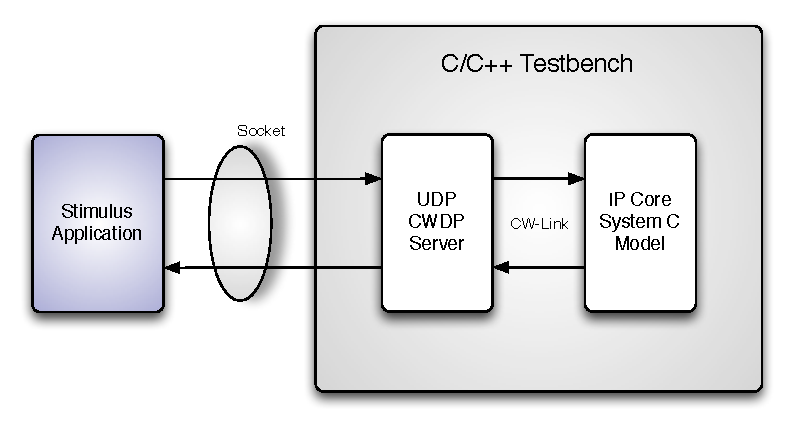
\includegraphics[width=9cm,center]{Diagrams/Simp-Diag.pdf}
  \caption{A UDP/CWDP cycle accurate simulator}\label{fig:udpserver}
\end{figure}


% use section* for acknowledgement
%\section*{Acknowledgment}






% trigger a \newpage just before the given reference
% number - used to balance the columns on the last page
% adjust value as needed - may need to be readjusted if
% the document is modified later
%\IEEEtriggeratref{8}
% The "triggered" command can be changed if desired:
%\IEEEtriggercmd{\enlargethispage{-5in}}

% references section

% can use a bibliography generated by BibTeX as a .bbl file
% BibTeX documentation can be easily obtained at:
% http://www.ctan.org/tex-archive/biblio/bibtex/contrib/doc/
% The IEEEtran BibTeX style support page is at:
% http://www.michaelshell.org/tex/ieeetran/bibtex/
%\bibliographystyle{IEEEtran}
% argument is your BibTeX string definitions and bibliography database(s)
%\bibliography{IEEEabrv,../bib/paper}
%
% <OR> manually copy in the resultant .bbl file
% set second argument of \begin to the number of references
% (used to reserve space for the reference number labels box)
\begin{thebibliography}{1}
%\bibitem{ncapat}
%J.~de~Sousa and N.~Lourenço and N.~Ribeiro and V.~Martins and R.~Martins \emph{NETWORK CORE ACCESS ARCHITECTURE} US PATENT 2008/0288652, 2008/05/15
%\bibitem{ncapateu}
%J.~de~Sousa and N.~Lourenço and N.~Ribeiro and V.~Martins and R.~Martins \emph{NETWORK CORE ACCESS ARCHITECTURE} EP PATENT 2003571/A2, 2008/12/17
%\bibitem{ieee802.3a}
%IEEE Standards Association \emph{IEEE STANDARD FOR ETHERNET} Section 1, Chapter 3 Media Access Control (MAC) frame and packet specifications
%\bibitem{ieee802.3b}
%IEEE Standards Association \emph{IEEE STANDARD FOR ETHERNET} Section 2, Chapter 22 Reconciliation Sublayer (RS) and Media Independent Interface (MII)
%\bibitem{rfc791}
%Jon Postel \emph{INTERNET PROTOCOL} RFC 791
%\bibitem{rfc826}
%Jon Postel \emph{USER DATAGRAM PROTOCOL} RFC 826
%\bibitem{Facedata}
%Coreworks \emph{FACEWORKS CWNET01 DATASHEET} 
%   publisher = {Coreworks},
%       month = {January},
%        year = {2008},
%}

\bibitem{ncapat}
J.~de~Sousa, N.~Lourenço, N.~Ribeiro, V.~Martins, and R.~Martins, ``Network
  core access architecture,'' Patent US 2008/0\,288\,652, 05 15, 2008.
  [Online]. Available: http://www.google.com/patents/US8019832

\bibitem{ncapateu}
------, ``Network core access architecture,'' Patent EP 2\,003\,571/A2, 12 17,
  2008. [Online]. Available: http://www.google.com/patents/EP2003571A2

\bibitem{ieee802.3b}
I.~S. Association, \emph{IEEE Standard for Ethernet}.\hskip 1em plus 0.5em
  minus 0.4em\relax IEEE, August 2012, ch. Section 2, Chapter 22 Reconciliation
  Sublayer (RS) and Media Independent Interface (MII).

\bibitem{ieee802.3a}
------, \emph{IEEE Standard for Ethernet}.\hskip 1em plus 0.5em minus
  0.4em\relax IEEE, August 2012, ch. Section 1, Chapter 3 Media Access Control
  (MAC) frame and packet specifications.

\bibitem{rfc2119}
S.~Bradner, ``Key words for use in rfcs to indicate requirement levels,''
  http://www.ietf.org/rfc/rfc2119.txt, March 1997.

\bibitem{rfc826}
D.~C. Plummer, ``An ethernet address resolution protocol,''
  http://www.ietf.org/rfc/rfc768.txt, November 1982.

\bibitem{rfc791}
J.~Postel, ``Internet protocol,'' http://www.ietf.org/rfc/rfc791.txt, September
  1981.

\bibitem{rfc768}
------, ``User datagram protocol,'' http://www.ietf.org/rfc/rfc826.txt, August
  1980.

\bibitem{Facedata}
Coreworks, \emph{FaceWorks CWnet01 Datasheet, Multi-purpose Autonomous Network
  Interface Core}.\hskip 1em plus 0.5em minus 0.4em\relax Coreworks, January
  2008.

\bibitem{veribench}
W.~Snyder, ``Verilog simulator benchmarks,''
  http://www.veripool.org/wiki/veripool/Verilog\_Simulator\_Benchmarks, March
  2011.

\bibitem{verilatorman}
W.~Snyder, ``Verilator 3.846 manual,''
  http://www.veripool.org/projects/verilator/wiki/Documentation, March 2013.

\bibitem{sniffer}
T.~Carstens, ``Sniffex, sniffer example of tcp/ip packet capture using
  libpcap,'' http://www.tcpdump.org/sniffex.c, June 2013.

\bibitem{pycrc}
T.~Pircher, ``Cyclic redundancy check (crc) calculator and c source code
  generator,'' http://www.tty1.net/pycrc/index\_en.html, April 2013.

\bibitem{gtkwave}
T.~Bybell, ``Gtkwave, waveform viewer,'' http://gtkwave.sourceforge.net, April
  2013.

\end{thebibliography}




% that's all folks
\end{document}


